\section{从无前缀安全PRF到完全安全PRF(方法3):CMAC}\label{sec:6-7}

上一节中介绍的两种无前缀编码方法都有问题。第一种方法产生的 MAC 是非流式的,而第二种方法对于长的消息需要对底层的 PRF 进行更多的计算。我们可以将无前缀编码进行随机化处理来进一步地改进设计。我们下面建立一个流式且安全的 PRF,除了底层的无前缀安全 PRF 之外,该设计不会引入任何额外的开销。图 \ref{fig:6-6} 展示了这样的 MAC,它比从加密 PRF 或者确定性编码得到的 MAC 都要优秀。这种方法被用于 NIST 的一种 MAC 标准,称为 CMAC,我们将在 \ref{sec:6-10} 节中介绍它。

\begin{figure}
  \centering
  \subfigure[应用于 CBC 的 $rpf$]{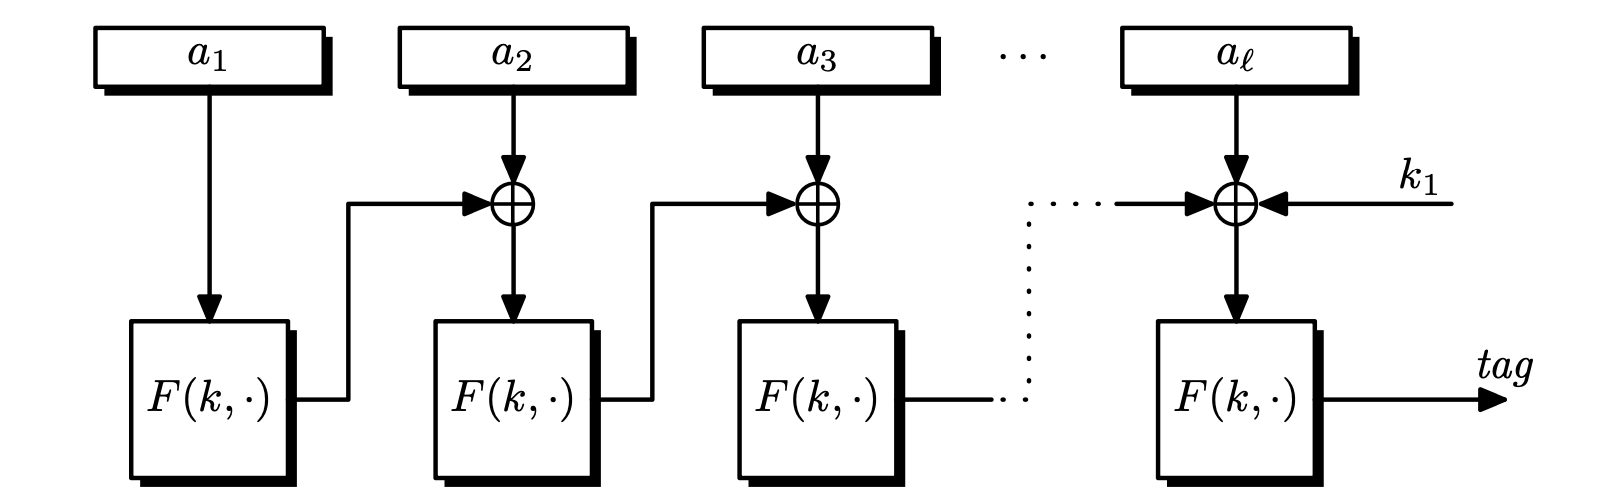
\includegraphics[width=0.8\linewidth]{figures/chapter6/fig6-a.png}}
  
  \subfigure[应用于级联的 $rpf$]{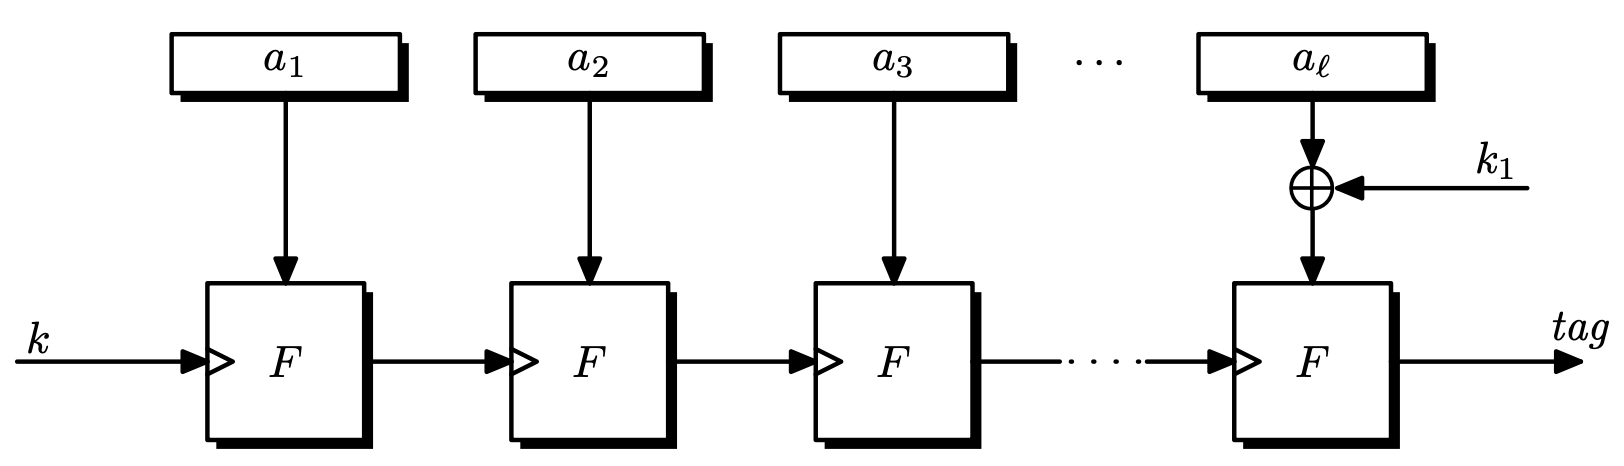
\includegraphics[width=0.8\linewidth]{figures/chapter6/fig6-b.png}}
  \caption{使用随机无前缀编码的安全 PRF}
  \label{fig:6-6}
\end{figure}

首先,为了叙述方便,我们引入一些符号:

\begin{definition}\label{def:6-5}
对于两个序列 $x,y\in\mathcal{X}^{\leq\ell}$,如果 $x$ 是 $y$ 的一个前缀,或者 $y$ 是 $x$ 的一个前缀,我们就记 $x\sim y$。
\end{definition}

\begin{definition}\label{def:6-6}
令 $\epsilon$ 是一个实数,满足 $0\leq\epsilon\leq1$。一个\textbf{随机性 $\epsilon$-无前缀 (randomized $\epsilon$-prefix-free)} 编码是一个函数 $rpf:\mathcal{K}\times\mathcal{M}\to\mathcal{X}^{\leq\ell}_{_{>0}}$,使得对于任意 $m_0,m_1\in\mathcal{M}$,$m_0\neq m_1$,我们都有:
\[
\Pr\big[rpf(k,m_0)\sim rpf(k,m_1)\big]\leq\epsilon
\]
这里的概率取决于从 $\mathcal{K}$ 中随机选取的 $k$。
\end{definition}

\noindent
请注意,$rpf(k,\cdot)$ 的像不需要是一个无前缀集合。然而,在不知道 $k$ 的情况下,很难找到 $m_0,m_1\in\mathcal{M}$ 使得 $rpf(k,m_0)$ 是 $rpf(k,m_1)$ 的真前缀(或者反之)。函数 $rpf(k,\cdot)$ 甚至不需要是一个单射。

\begin{snote}[一个简单的 $rpf$。]
令 $\mathcal{K}:=\mathcal{X}$,$\mathcal{M}:=\mathcal{X}^{\leq\ell}_{_{>0}}$。定义:
\[
rpf(k,(a_1,\dots,a_v))=(a_1,\dots,a_{v-1},(a_v\oplus k))\in\mathcal{X}^{\leq\ell}_{_{>0}}
\]
不难发现 $rpf$ 是一个随机性 $({1}/{|\mathcal{X}|})$-无前缀编码。令 $m_0,m_1\in\mathcal{M}$,并且 $m_0\neq m_1$。假设 $|m_0|=|m_1|$。那么很明显,对于所有 $k$ 的选择,$rpf(k,m_0)$ 和 $rpf(k,m_1)$ 都是长度相同的不同序列,所以两者都不可能是对方的前缀。接下来,假设 $|m_0|<|m_1|$。如果 $v:=|rpf(k,m_0)|$,那么很显然,当且仅当:
\[
m_0[v-1]\oplus k=m_1[v-1]
\]
时,$rpf(k,m_0)$ 才是 $rpf(k,m_1)$ 的一个真前缀。然而,在随机选择 $k$ 的情况下,上式成立的概率是 ${1}/{|\mathcal{X}|}$,这符合要求。最后,对于 $|m_0|>|m_1|$ 的情况,可以用一个对称的论证来处理。
\end{snote}

\begin{snote}[使用 $rpf$。]
令 $PF$ 是一个定义在 $(\mathcal{K},\mathcal{X}^{\leq\ell},\mathcal{Y})$ 上的无前缀安全 PRF,且 $rpf:\mathcal{K}_1\times\mathcal{M}\to\mathcal{X}^{\leq\ell}_{_{>0}}$ 是一个随机化的无前缀编码。定义派生出的 PRF $F$ 为:
\begin{equation}\label{eq:6-21}
F\big((k,k_1),\,m\big):=PF\big(k,\,rpf(k_1,m)\big)
\end{equation}
那么,$F$ 就定义在 $(\mathcal{K}\times\mathcal{K}_1,\mathcal{M},\mathcal{Y})$ 上。我们可以得到以下定理,它与定理 \ref{theo:6-8} 类似。
\end{snote}

\begin{theorem}\label{theo:6-9}
如果 $PF$ 是一个无前缀安全的 PRF,$\epsilon$ 可忽略不计,并且 $rpf$ 是一个随机性 $\epsilon$-无前缀编码,则式 \ref{eq:6-21} 中定义的 $F$ 是一个安全的 PRF。
\begin{quote}
特别地,对于每个按照攻击游戏 \ref{game:4-2} 攻击 $F$ 的 PRF 对手 $\mathcal{A}$,假设它最多能够向其挑战者发起 $Q$ 次查询,则必然存在两个按照攻击游戏 \ref{game:4-2} 攻击 $PF$ 的无前缀 PRF 对手 $\mathcal{B}_1$ 和 $\mathcal{B}_2$,使得 $\mathcal{B}_1$ 和 $\mathcal{B}_2$ 都是围绕 $\mathcal{A}$ 的基本包装器,满足:
\end{quote}
\begin{equation}\label{eq:6-22}
{\rm PRF}\mathsf{adv}[\mathcal{A},F]\leq
{\rm PRF^{pf}}\mathsf{adv}[\mathcal{B}_1,PF]+{\rm PRF^{pf}}\mathsf{adv}[\mathcal{B}_2,PF]+{Q^2\epsilon}/{2}
\end{equation}
\end{theorem}

\begin{proof}[证明思路]
如果对手对于 $F$ 的输入集能够产生对于 $PF$ 的无前缀输入集,那么对手看到的就只是一些看起来很随机的输出。此外,如果对手看到的是随机的输出,它就没有得到关于 $rpf$ 的密钥 $k_1$ 的任何有效信息,这就确保 $PF$ 的输入集确实(以压倒性的概率)是无前缀的。不幸的是,上述思路会导致一个循环论证。我们将在下面的证明中介绍打破这种循环论证的方法。
\end{proof}

\begin{proof}
不失一般性,我们假设 $\mathcal{A}$ 从未发出过两次相同的查询。我们将证明组织成由三个游戏构成的一个序列。对于 $j=0,1,2$,我们令 $W_j$ 是 $\mathcal{A}$ 在游戏 $j$ 结束时输出 $1$ 的事件。

\vspace{5pt}

\noindent\textbf{游戏$\mathbf{0}$}。
在 PRF 攻击游戏 \ref{game:4-2} 的实验 $0$ 中,挑战者就 $F$ 进行如下操作:

\vspace{5pt}

\hspace*{5pt} 选取 $k\overset{\rm R}\leftarrow\mathcal{K}$,$k_1\overset{\rm R}\leftarrow\mathcal{K}_1$\\
\hspace*{26pt} 当从 $\mathcal{A}$ 处收到签名查询 $m_i\in\mathcal{M}$ ($i=1,2,\dots$) 时:\\
\hspace*{50pt} 令 $x_i\leftarrow rpf(k_1,m_i)\in\mathcal{X}^{\leq\ell}_{_{>0}}$\\
\hspace*{50pt} 令 $y_i\leftarrow PF(k,x_i)$\\
\hspace*{50pt} 将 $y_i$ 发送给 $\mathcal{A}$

\vspace{5pt}

\noindent\textbf{游戏$\mathbf{1}$}。
我们修改游戏 $0$ 中的挑战者,以确保对 $PF$ 的所有查询都是无前缀的。回顾一下符号 $x\sim y$,它表示 $x$ 是 $y$ 的前缀,或者 $y$ 是 $x$ 的前缀。

\vspace{5pt}

\hspace*{5pt} 选取 $k\overset{\rm R}\leftarrow\mathcal{K}$,$k_1\overset{\rm R}\leftarrow\mathcal{K}_1$,$r_1,\dots,r_Q\overset{\rm R}\leftarrow\mathcal{Y}$\\
\hspace*{26pt} 当从 $\mathcal{A}$ 处收到签名查询 $m_i\in\mathcal{M}$ ($i=1,2,\dots$) 时:\\
\hspace*{50pt} 令 $x_i\leftarrow rpf(k_1,m_i)\in\mathcal{X}^{\leq\ell}_{_{>0}}$\\
\hspace*{1pt} ($1$)
\hspace*{28.5pt} 如果存在某个 $j<i$ 使得 $x_i\sim x_j$:\\
\hspace*{75pt} 则令 $y_i\leftarrow r_i$\\
\hspace*{1pt} ($2$)
\hspace*{53.5pt} 否则令 $y_i\leftarrow PF(k,x_i)$\\ % 21.5pt deducted
\hspace*{50pt} 将 $y_i$ 发送给 $\mathcal{A}$

\vspace{5pt}

\noindent
令 $Z_1$ 为在游戏 $1$ 中的某个时刻,行 ($1$) 中的条件成立的事件。显然,在事件 $Z_1$ 发生之前,游戏 $1$ 和游戏 $2$ 的进程是完全相同的;特别地,当且仅当 $W_1\land\bar{Z}_1$ 发生时,$W_0\land\bar{Z}_1$ 才会发生。因此,基于差分引理(定理 \ref{theo:4-7}),我们得到:
\begin{equation}\label{eq:6-23}
\big\lvert\Pr[W_1]-\Pr[W_0]\big\rvert\leq\Pr[Z_1]
\end{equation}
不幸的是,在这一点上,我们还不能完全约束 $\Pr[Z_1]$。当分析进行到这一阶段时,我们还不能说明对 $PF$ 的评估在行 ($2$) 不会泄漏关于 $k_1$ 的信息。这些信息可能可以帮助 $\mathcal{A}$ 促使事件 $Z_1$ 发生。这就是我们上面提到的循环论证的问题。为了客服这一问题,我们把对 $Z_1$ 的分析推迟到下一个游戏。

\vspace{5pt}

\noindent\textbf{游戏$\mathbf{2}$}。
现在,与往常一样,我们打出``PRF牌",用一个真随机函数取代函数 $PF(k,\cdot)$。这是合理的,因为从构造上来看,在游戏 $1$ 中,$PF(k,\cdot)$ 的输入集是无前缀的。为了实现这一修改,我们可以简单地将标有 ($2$) 的一行替换为:

\vspace{5pt}

\hspace*{-19pt} ($2$)
\hspace*{53.5pt} 否则令 $y_i\leftarrow PF(k,x_i)$

\vspace{5pt}

\noindent
做了这样的修改后,我们可以看到,无论行 ($1$) 中的条件是否成立,$y_i$ 都会被分配一个随机值 $r_i$。

现在,令 $Z_2$ 表示在游戏 $2$ 中的某个时刻,行 ($1$) 中的条件成立的事件。不难得到,对于有效的无前缀 PRF 对手 $\mathcal{B}_1$ 和 $\mathcal{B}_2$,有:
\begin{equation}\label{eq:6-24}
\big\lvert\Pr[Z_1]-\Pr[Z_2]\big\rvert\leq{\rm PRF^{pf}}\mathsf{adv}[\mathcal{B}_1,F]
\end{equation}
和:
\begin{equation}\label{eq:6-25}
\big\lvert\Pr[W_1]-\Pr[W_2]\big\rvert\leq{\rm PRF^{pf}}\mathsf{adv}[\mathcal{B}_2,F]
\end{equation}
成立。这两个对手基本上是一样的,只是当行 ($1$) 中的条件成立时,$\mathcal{B}_1$ 就会输出 $1$,而 $\mathcal{B}_2$ 则会输出 $\mathcal{A}$ 所输出的任何结果。

此外,在游戏 $2$ 中,$k_1$ 的值显然与 $\mathcal{A}$ 的查询无关,因此利用 $rpf$ 的 $\epsilon$-无前缀属性,根据联合约束,我们可以得到:
\begin{equation}\label{eq:6-26}
\Pr[Z_2]\leq{Q^2\epsilon}/{2}
\end{equation}

最后,对 $\mathcal{A}$ 来说,游戏 $2$ 完美地模拟了 ${\rm Funs}[\mathcal{M},\mathcal{Y}]$ 中的一个随机函数。因此,游戏 $2$ 与就 $F$ 的攻击游戏 \ref{game:4-2} 中的实验 $1$ 是相同的,因此:
\begin{equation}\label{eq:6-27}
\big\lvert\Pr[W_0]-\Pr[W_2]\big\rvert={\rm PRF}\mathsf{adv}[\mathcal{A},F]
\end{equation}
现在,结合式 \ref{eq:6-23},\ref{eq:6-24},\ref{eq:6-25},\ref{eq:6-26} 和 \ref{eq:6-27},该定理得证。
\end{proof}